\documentclass{bioinfo}
\copyrightyear{2021} \pubyear{2021}

\access{Advance Access Publication Date: Day Month Year}
\appnotes{Manuscript Category}

\usepackage{natbib}


\begin{document}
\firstpage{1}

\subtitle{Sequence analysis}

\title[VPsearch]{VPsearch: fast exact sequence similarity search for genomic sequences}
\author[Vankerschaver \textit{et~al}.]{%
  J. Vankerschaver$^{\text{\sfb 2,3,}*}$, R. Cardwell, R. Kern$^{\text{\sfb 1}}$, S.J. Kern$^{\text{\sfb 1}}$,
  P. Zahemszky$^{\text{\sfb 1}}$}
\address{$^{\text{\sf 1}}$Enthought Inc., 200 W Cesar Chavez, Austin, TX 78701, United States \\
  $^{\text{\sf 2}}$ Center for Biosystems and Biotech Data Analysis, Ghent University Global Campus, Republic of Korea \\
  $^{\text{\sf 3}}$ Department of Applied Mathematics, Computer Science and Statistics, Ghent University, Belgium}

\corresp{$^\ast$To whom correspondence should be addressed.}

\history{Received on XXXXX; revised on XXXXX; accepted on XXXXX}

\editor{Associate Editor: XXXXXXX}

\abstract{%
  \textbf{Summary:} Similarity search in databases of nucleotide sequences is a
  fundamental task for the determination of new organisms and the functional
  elucidation of existing genomes. Here we present VPsearch, an open-source,
  multithreaded command-line application for fast genomic sequence lookup which
  matches the lookup accuracy of existing tools like BLAST and
  ggsearch36 but offers greatly improved lookup speed.  \\
  \textbf{Availability and implementation:} VPsearch is implemented in Python 3
  and is available from the Python Package Index (\texttt{pip install
    vpsearch}) or as a Docker/Singularity image. The source code is licensed
  under the BSD
  license and can be retrieved from \texttt{https://github.com/enthought/vpsearch}.  \\
  \textbf{Contact:} Joris.Vankerschaver@ghent.ac.kr \\
  \textbf{Supplementary information:} Supplementary data are available at
  \textit{Bioinformatics} online.}

\maketitle

% Paper %%%%%%%%%%%%%%%%%%%%%%%%%%%%%%%%%%%%%%%%%%%%%%%%%%%%%%%%%%%%%%%%%%%%%%%

\vspace*{-0.5cm}
\section{Introduction}

Similarity search, \emph{i.e.} finding an approximate match from a database of
known nucleotide sequences given an unknown query sequence, is a central task
in the taxonomic determination and functional understanding of newly sequenced
organisms. As databases of known, curated sequences and the number of unknown
sequences continue to grow exponentially, tools that can organize genomic data
at scale and make it efficiently accessible are of fundamental importance.

Over the years, a number of tools for similarity search have improved upon
BLAST in terms of lookup speed and accuracy. Some of these, such as the FASTA
tool suite (\cite{2016-pearson-FindingProteinNucleotide}), provide rapid
protein or nucleotide similarity search based on sequence content
alone. Others, such as the RDP classifier
(\cite{2007-wang-NaiveBayesianClassifier}) for microbiome analysis, take
taxonomic information or other domain-specific information into account to
improve classification sensitivity or to provide additional confidence
measures. For whole-genome sequences, data structures for approximate
similarity search have been adopted to improve sequence lookup speed
(\cite{2019-marcais-SketchingSublinearData}).

In this paper we present VPsearch, a light-weight Python package and
command-line tool to organize nucleotide sequences into a so-called
\emph{vantage point tree} (\cite{1991-uhlmann-SatisfyingGeneralProximity},
\cite{1993-yianilos-DataStructuresAlgorithms}). This data structure allows for
similarity searches that use a number of lookups proportional to the logarithm
of the size of the database (rather than scanning through the database in
linear fashion), and hence greatly speeds up similarity search queries. We show
that for short sequences (such as the 16S rRNA gene used in bacterial
classification) VPsearch outperforms both BLAST (7x speedup) and ggsearch36
from the FASTA suite (27x speedup) without any loss in accuracy.

Vantage point trees were used by
\cite{2016-defreitas-GEMINIComputationallyefficientSearch} for (numerical) gene
expression data. To the best of our knowledge, this is the first time that
vantage point trees have been used for nucleotide sequences.

\vspace*{-0.5cm}
\section{Software description}

The VPsearch tool is implemented in Python, using Cython for performance-critical sections.
It outputs similarity search results in the ``BLAST-6''
tabular format used by BLAST, Diamond, the FASTA tool suite and others, so that
VPsearch can be used as a drop-in replacement for any of these tools. VPsearch
is able to return the $k$ most similar sequences for a given query, not just
the most similar match, and is fully multithreaded.

In order to build and query a vantage point tree, VPsearch requires a measure
of similarity between nucleotide sequences. Such a similarity measure can be
computed via the Needleman-Wunsch sequence alignment algorithm, and an
expression is given in the supplementary material. To compute the
Needleman-Wunsch alignment efficiently, VPsearch uses the Parasail library
(\cite{2016-daily-ParasailSIMDLibrary}) which offers an optimized, SIMD-enabled
implementation of the Needleman-Wunsch algorithm (among others).

The vantage point tree is built in two stages. In the first, a tree is built by
recursively choosing a representative sequence as vantage point and subdividing
the remaining sequences into the 50\% most similar and 50\% least similar
sequences. The construction is then repeated recursively on these two
subcollections, resulting in a binary search tree. In the second stage, the
tree is converted into an array of left/right pointers and vantage point
distances. This representation is compact and cache-friendly, and is saved to disk for
subsequent querying.

One important caveat is that VPsearch uses global-to-global alignment and
therefore requires a database and query set of clean sequences that start and
end in the same, homologous locations. For 16S and other amplicon sequences
this is usually not a problem, since the region of interest (e.g. the
hypervariable v4 region used for taxonomic determination) is usually bracketed
by conserved regions which are not amplified and sequenced, or which can be
trimmed using a primer-cutting tool. Note that ggsearch36 has the same
limitation, while local alignment based tools like Blast+ do not.

\vspace*{-0.5cm}
\section{Case study}

We compared the performance of VPsearch with two standard tools for sequence
lookup: Blast+, a standard tool that is optimized for inexact but fast sequence
lookup via the matching sequence pair heuristic
(\cite{1990-altschul-BasicLocalAlignment}), and ggsearch36, part of the FASTA
suite (\cite{2016-pearson-FindingProteinNucleotide}), which relies on exact
alignment to achieve higher accuracy at the cost of greatly increased lookup
times. We show that VPsearch manages to combine the good aspects of both tools,
while avoiding the drawbacks.

To test the performance of VPsearch under realistic conditions, we used the
Mothur SOP dataset (\cite{2013-kozich-DevelopmentDualIndexSequencing})
consisting of paired-end (2x 250bp) MiSeq-sequenced reads of the v4
hypervariable region of the 16S rNA gene from gut samples harvested from mice.
This dataset was prepared using the Dada2 protocol
(\cite{2016-callahan-DADA2HighresolutionSample}), resulting in 232 amplicon
sequence variants (ASV). For taxonomic assignments, we used Version 138 of the
Silva database (\cite{2013-quast-SILVARibosomalRNA}). The database was
processed by excising the v4 region and removing duplicate sequences, resulting
in a database of 230,013 sequences with known taxonomies.

Benchmarking was done on a c5.xlarge instance (Amazon Web Services) with 4 CPU
cores (Intel Xeon, 3.5 GHz) and 8GB of RAM. The scripts used for database
preparation and benchmarking are available from GitHub
(\texttt{https://github.com/jvkersch/vpsearch-paper}) and as part of the
supplementary material.

\subsection{Taxonomic accuracy}

For each ASV, we compared the top matches (ranked by alignment score) between
VPsearch, ggsearch36, and Blast+. Out of 232 ASVs there is one sequence where
the taxonomic assignment differs between ggsearch36 and VPsearch, due to a
small difference in how the alignment parameters are chosen for both
algorithms. Both algorithms identify the ASV as being in the family of
\emph{Lachnospiraceae}, with the difference on the genus level. Between
VPsearch and Blast+, there are three difference assignments, due to the fact
that several sequences in the database present an equally plausible match for
the query sequence.

\subsection{Improvements in lookup time}

To assess the taxonomic lookup time in function of the database size, we took
five random subsets of the Silva database (consisting of 100, 1000, 10,000, 100,000,
and all 230031 sequences) and measured the time needed to look up the 232 ASVs
for each tool. We repeated each measurement 7 times and took the average. On
the full Silva database, VPsearch is clearly the fastest (20s total lookup
time), compared to Blast+ (157s) and ggsearch (561.3s).

For Blast+ and ggsearch36, the total lookup time scales linearly with the size
of the database, whereas for VPsearch the scaling is logarithmical (in other
words, making the database 10 times larger adds a constant factor to the total
lookup time). We therefore believe that VPsearch will continue to be an accurate
yet performant lookup tool, even as sizes of genomic databases continue to increase.

\begin{figure}
  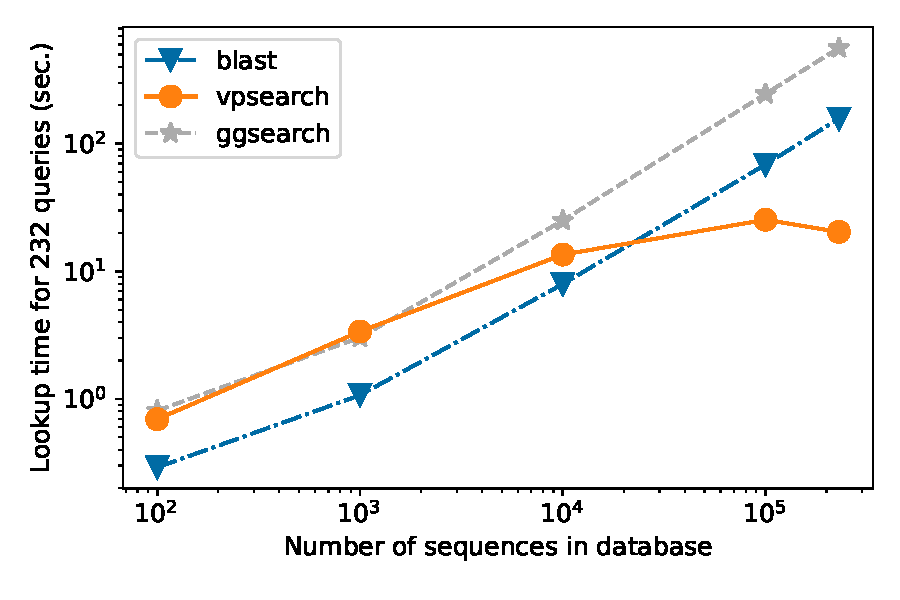
\includegraphics[scale=0.5]{execution-time.pdf}
  \caption{Sequence lookup time for 232 sequences as a function of the size of
    the database. For small databases (less than 10,000 sequences), VPsearch
    performs comparably to Blast+ and ggsearch36. For realistic databases
    (consisting of more than 50,000 sequences), the VPsearch lookup times
    scales logarithmically as the size of the database increases.}
\end{figure}

\vspace*{-0.7cm}
\section*{Acknowledgements}

JV is supported by the ``Bijzondere Onderzoeksfonds'' (BOF) of Ghent University. We
would like to thank Jun Isayama and Yuko Kiridoshi for stimulating discussions,
and Homin Park for help in setting up the computational infrastructure.

% Bibliography %%%%%%%%%%%%%%%%%%%%%%%%%%%%%%%%%%%%%%%%%%%%%%%%%%%%%%%%%%%%%%%%

\vspace*{-0.5cm}
\bibliography{vpsearch-paper}
\bibliographystyle{natbib}

\end{document}
